\documentclass[hide notes,intlimits]{beamer}

\mode<presentation>
{
  \usetheme[footline]{UAFshade}
  \setbeamercovered{transparent}
}

% load packages
\usepackage{tikz}
\usetikzlibrary{shapes,arrows,shadows}

\usepackage[english]{babel}
\usepackage[latin1]{inputenc}
\usepackage[T1]{fontenc}
\usepackage{lmodern}
\usepackage{multimedia}
%\usepackage{hyperref}

% Some useful commands (from ELB)
\newcommand{\bD}{\mathbf{D}}
\newcommand{\bbf}{\mathbf{f}}
\newcommand{\bF}{\mathbf{F}}
\newcommand{\bg}{\mathbf{g}}
\newcommand{\bn}{\mathbf{n}}
\newcommand{\bq}{\mathbf{q}}
\newcommand{\bT}{\mathbf{T}}
\newcommand{\bu}{\mathbf{u}}
\newcommand{\bU}{\mathbf{U}}
\newcommand{\bv}{\mathbf{v}}





\graphicspath{{figures/}}

\newenvironment{transbox}{%

\begin{tikzpicture}
\node[drop shadow,rounded corners,text width=\textwidth,fill=white, fill opacity=0.75,text opacity=1] \bgroup
}{
\egroup;\end{tikzpicture}} 

\setbeamercolor{boxed}{fg=black,bg=uaf yellow}


% title page
\title[Glacier Dynamics] % (optional, use only with long paper titles)
{Dynamics of Glaciers}
\subtitle{McCarthy Summer School}

\author[Aschwanden] % (optional, use only with lots of authors)
{Andy Aschwanden}
% - Give the names in the same order as the appear in the paper.
% - Use the \inst{?} command only if the authors have different
%   affiliation.

\institute[GI] % (optional, but mostly needed)
{
  %
  Geophysical Institute\\
  University of Alaska Fairbanks, USA
}
% - Use the \inst command only if there are several affiliations.
% - Keep it simple, no one is interested in your street address.

\date{August 2014}

\titlegraphic{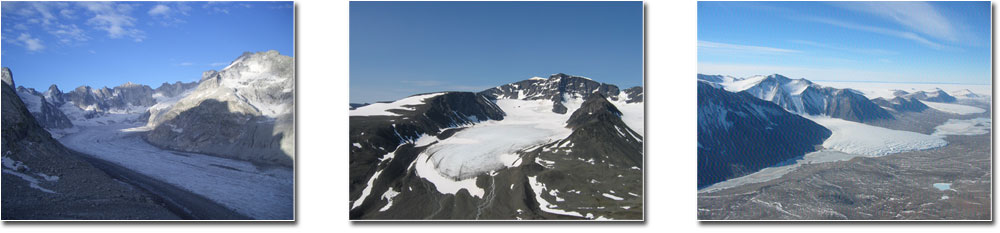
\includegraphics[width=10cm]{glaciers3}}


\subject{Glaciers}

\begin{document}

\AtBeginSection[]
{
  \begin{frame}<handout:0>
    \frametitle{Outline}
    \tableofcontents[sectionstyle=show/shaded,subsectionstyle=hide]
  \end{frame}
}


\setbeamertemplate{background canvas}
  {
     \tikz{\node[inner sep=0pt,opacity=1.0] {\includegraphics[width=\paperwidth]{uaf_beamer_shade_bg}};}
} 

% insert titlepage
\begin{frame}
  \titlepage
\end{frame}

\setbeamertemplate{background canvas}
{
%
} 

\begin{frame}
  \frametitle{Overview}
    \begin{itemize}
    \item \alert{selected} examples of glacier flow, using concepts from
      Continuum Mechanics
    \item leave out boundary conditions
    \item no tensors, yeah
    \end{itemize}
\end{frame}

\begin{frame}
  \frametitle{What is a glacier?}
  \centering{
    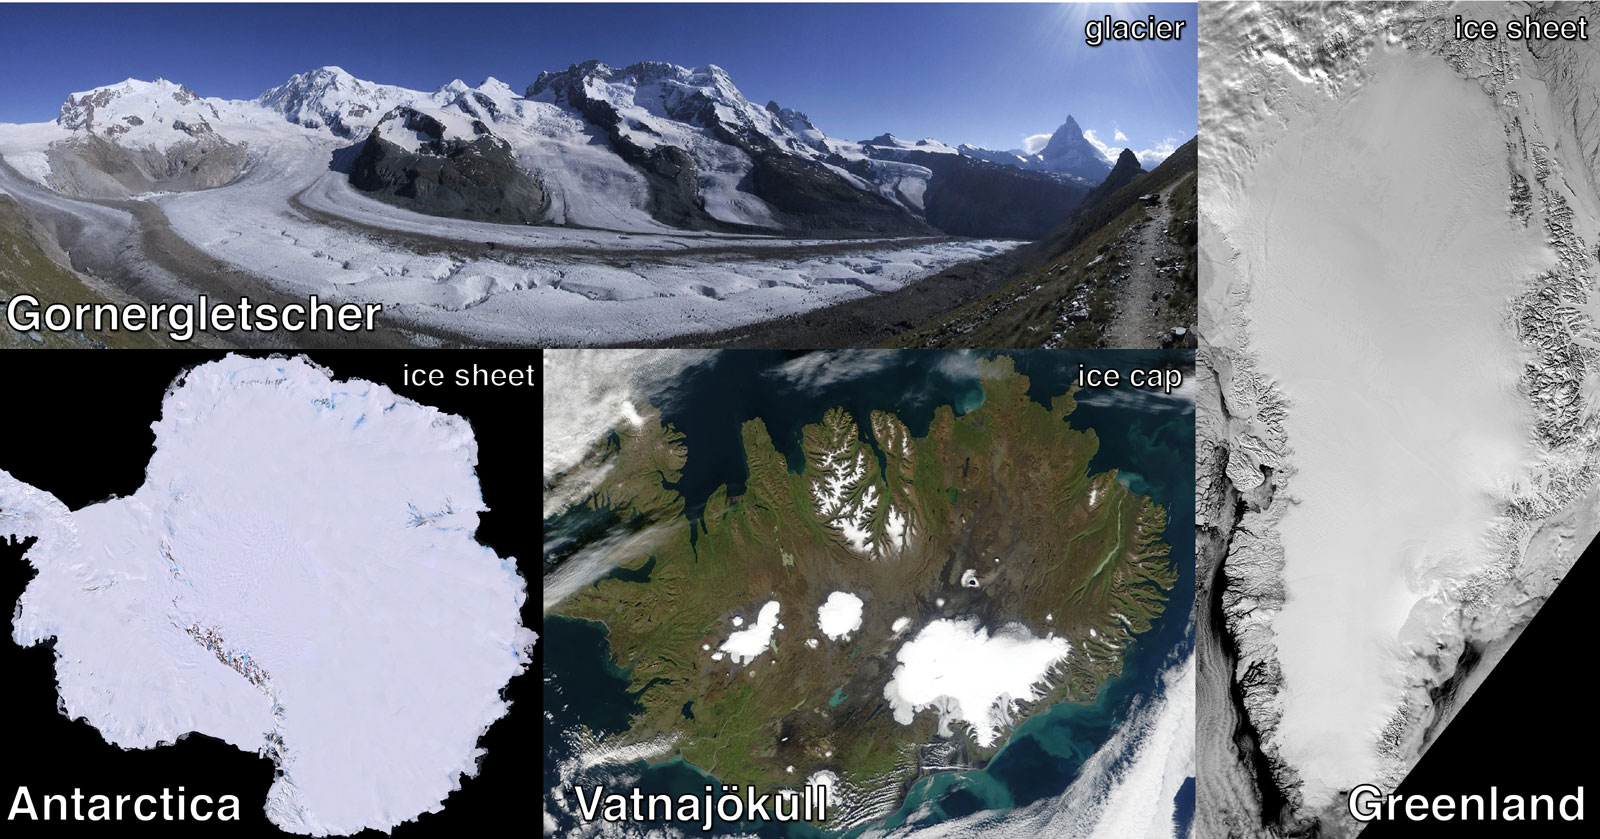
\includegraphics[width=.85\textwidth]{landice}
  }
  \begin{itemize}
  \item Glaciers flow slowly under their own weight
  \end{itemize}
  \note[itemize]{
    \item glaciers are the landice part of the cryosphere
}
\end{frame}

\begin{frame}
  \frametitle{Glacier flow}
  \begin{figure}
    \scriptsize{speeds by Evan Burgess (Wrangell) and Roman Motyka (Jakobshavn)}
    \includegraphics[width=.95\textwidth]{speeds-scale}
  \end{figure}
  \begin{itemize}
    \item observed speeds range from 20\,m\,a$^{-1}$ for a valley glacier to 15\,km\,a$^{-1}$
  \end{itemize}
  \note[itemize]{
}
\end{frame}

\setbeamertemplate{background canvas}
  {
     \tikz{\node[inner sep=0pt,opacity=1.0] {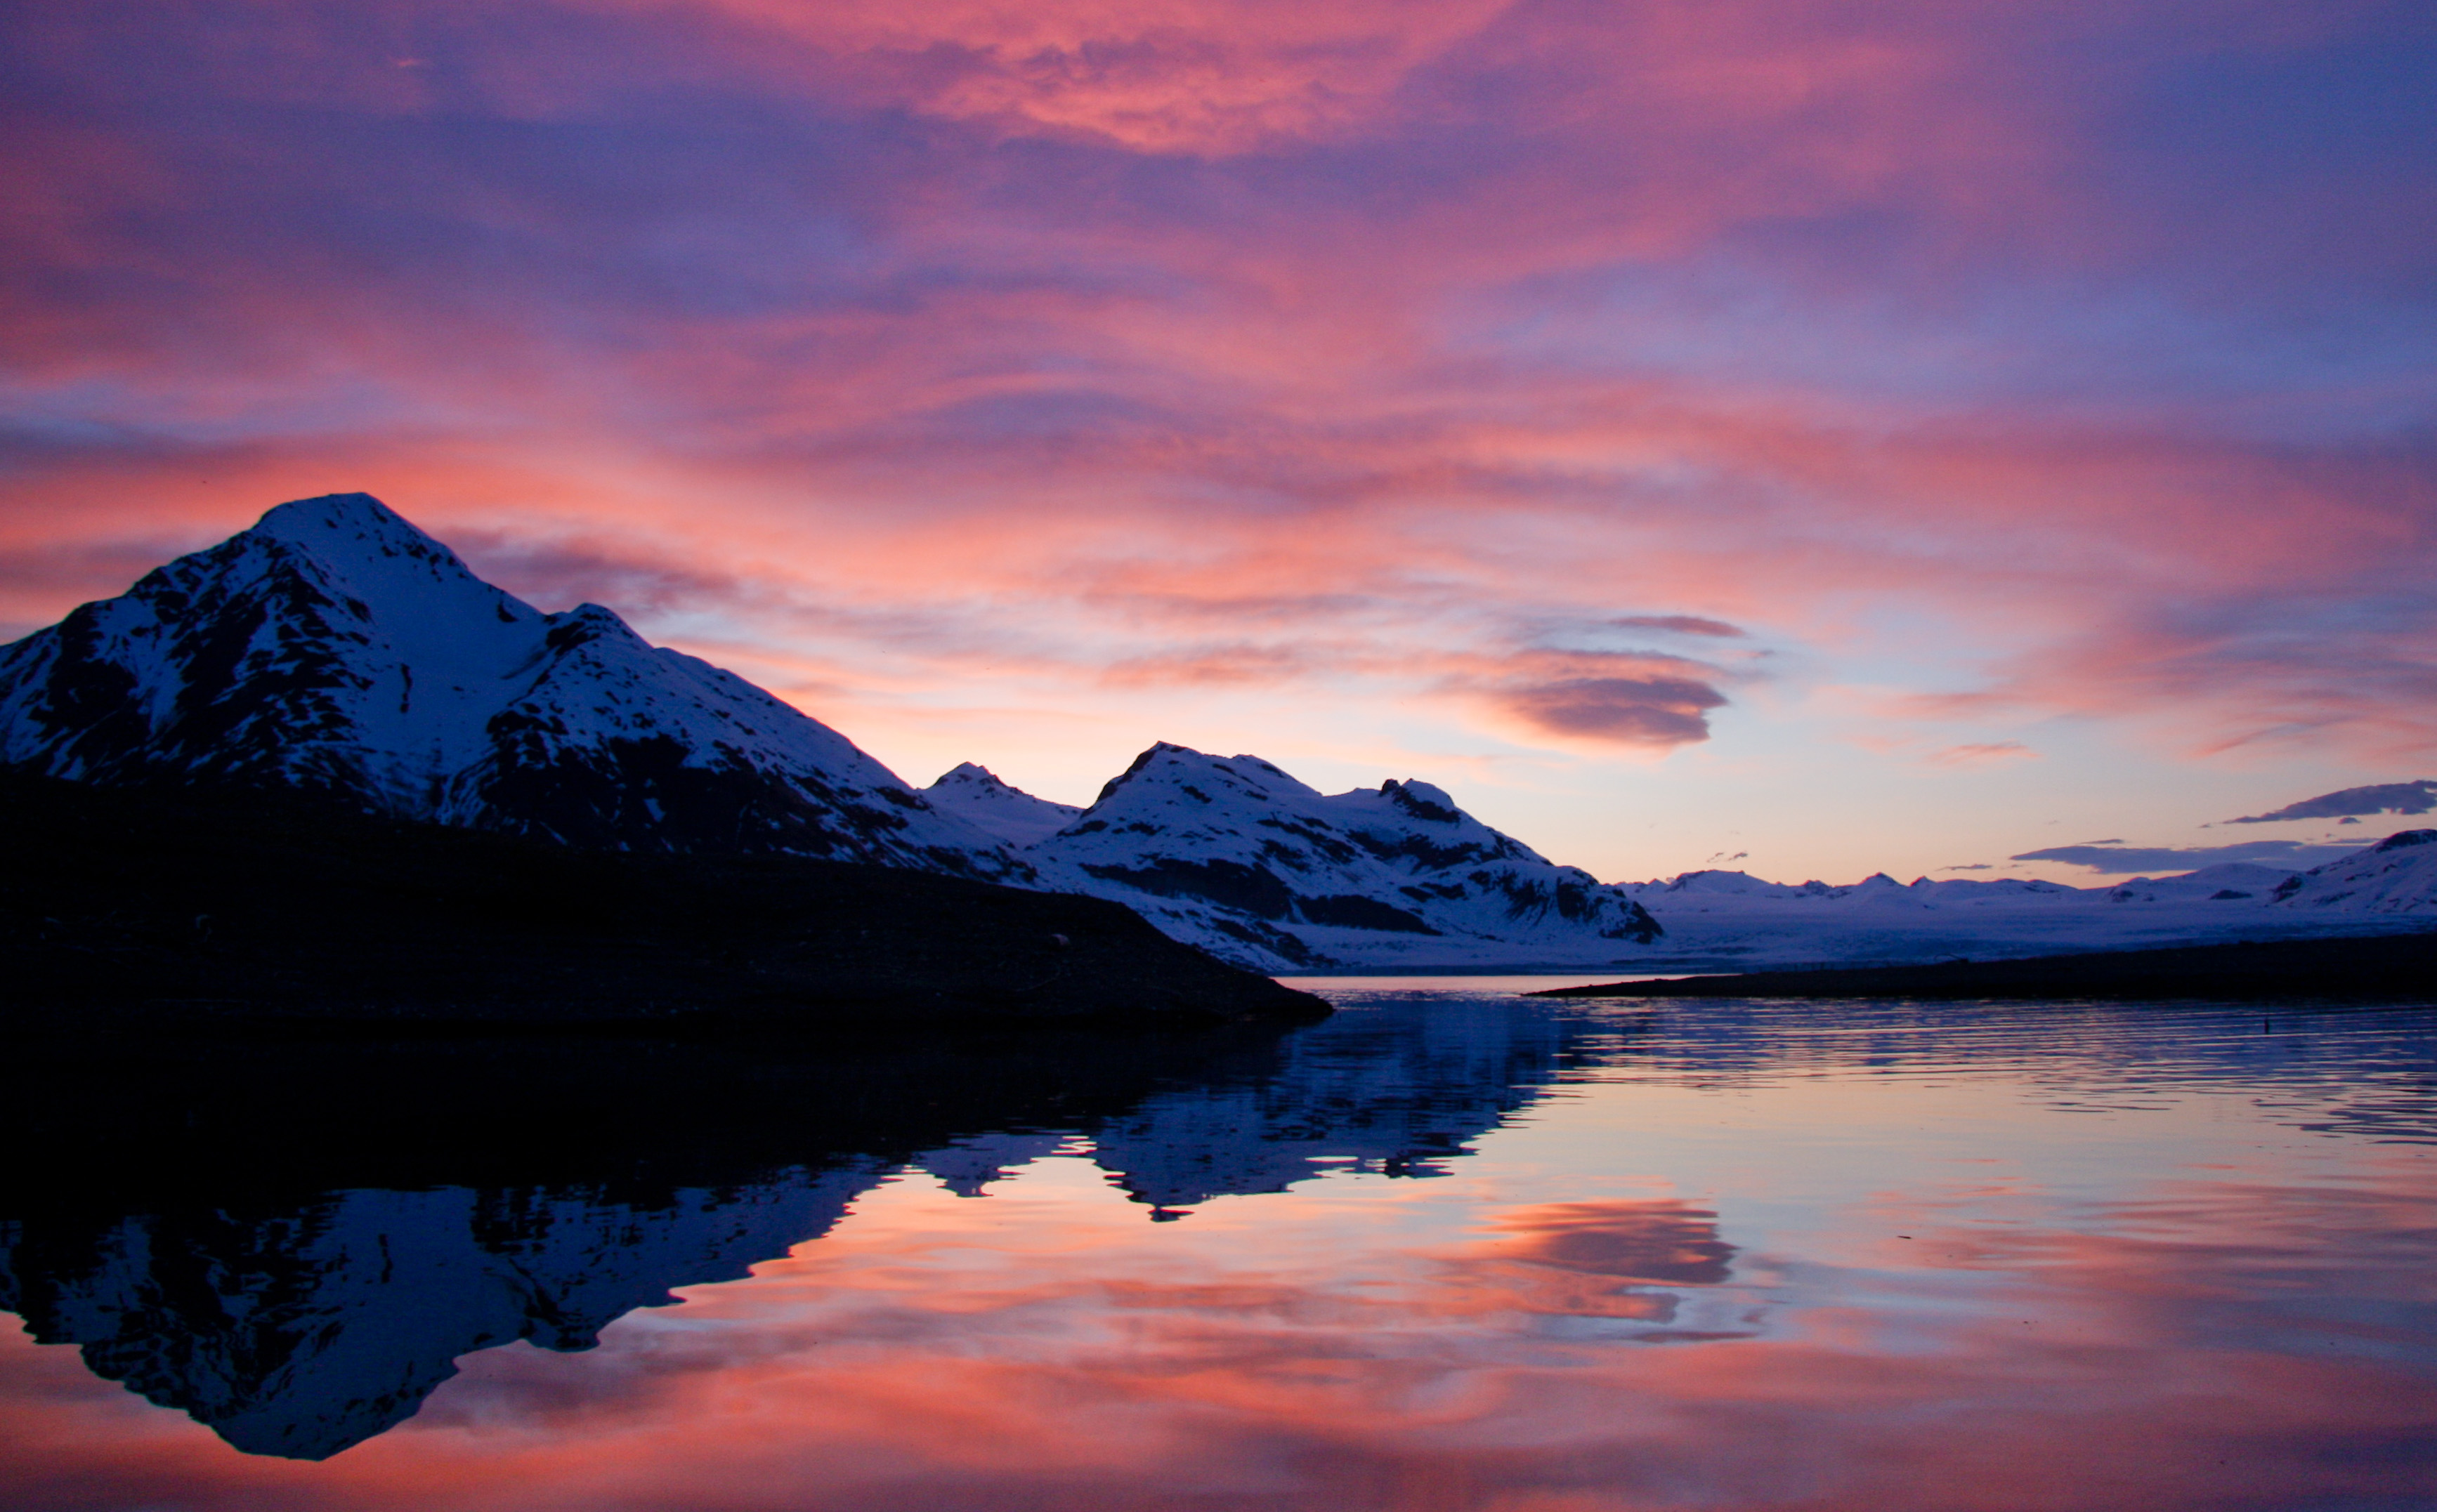
\includegraphics[height=
\paperheight,width=\paperwidth]{yakutat_sunset}};}
} 

\begin{frame}[plain] % not in the handout
  \begin{columns}
    \column[C]{7.5cm}
  \begin{transbox}
    ``The tradition of glacier studies that we inherit draws upon two great legacies of the eighteenth and nineteenth centuries: classical physics and romatic enthusiasm for Nature.\\[.25em]
\ldots It is easy to undervalue the romantic contribution, but in glaciology, it would be a mistake to do so'' \\[.5em]
\emph{Garry Clark, J. Glaciol., 1987)}
  \end{transbox}
\end{columns}
\end{frame}


\setbeamertemplate{background canvas}
{
%
} 


\begin{frame}
  \frametitle{How does a glacier move?}
  \centering{
    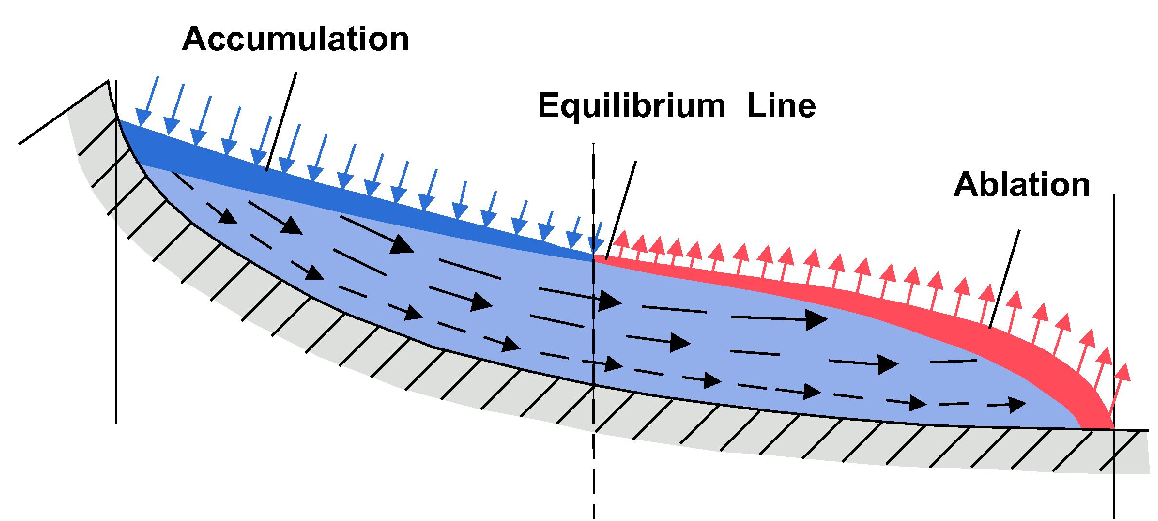
\includegraphics[width=.65\textwidth]{flow_acc_abl}
  }
  \begin{block}{In a nut shell:}
    \begin{itemize}
    \item Well-described by continuum mechanics (Martin's lecture on Thursday)
    \item The ice can deform as a viscous fluid
    \item The ice can slide over its substrate
    \end{itemize}
  \end{block}
\end{frame}

\begin{frame}
  \frametitle{Water plays an important role}
  \begin{figure}
    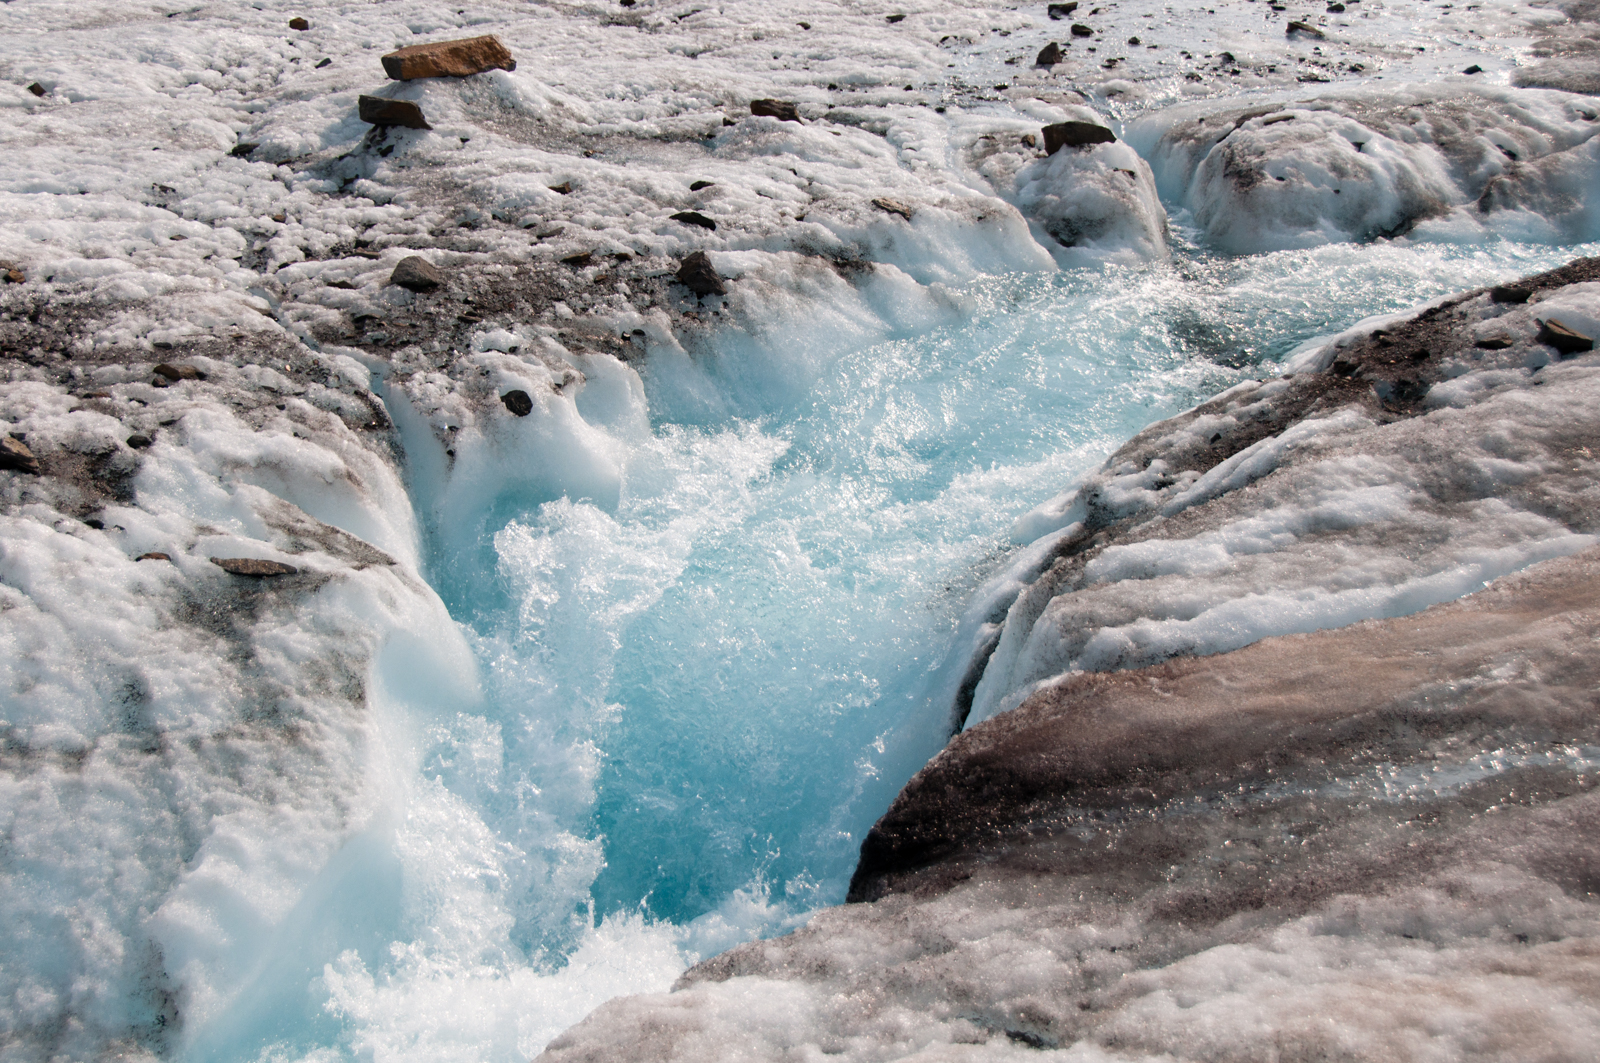
\includegraphics[height=4cm]{black-rapids-1} \vspace{0.25em}
    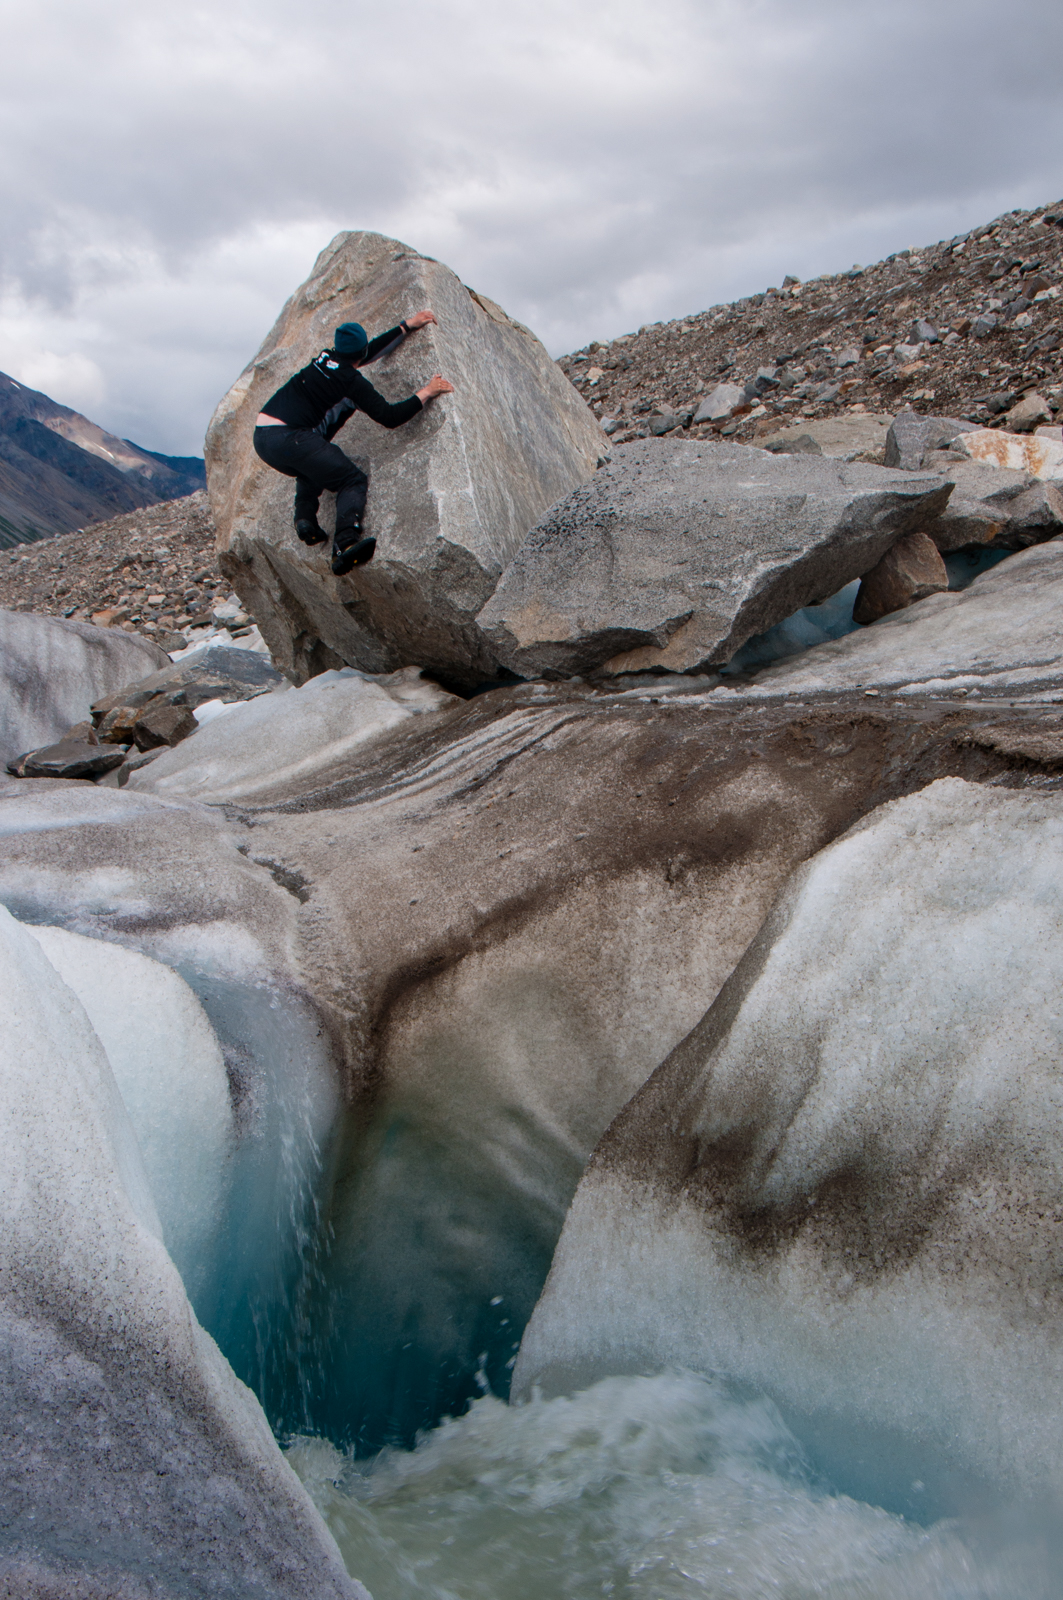
\includegraphics[height=4cm]{black-rapids-2}
  \end{figure}
  \begin{block}{Rule of thumb}
    \begin{itemize}
    \item whenever something interesting happens in a glacier, liquid water is involved
    \end{itemize}
  \end{block}
\end{frame}

\setbeamertemplate{background canvas}
  {
     \tikz{\node[inner sep=0pt,opacity=0.60] {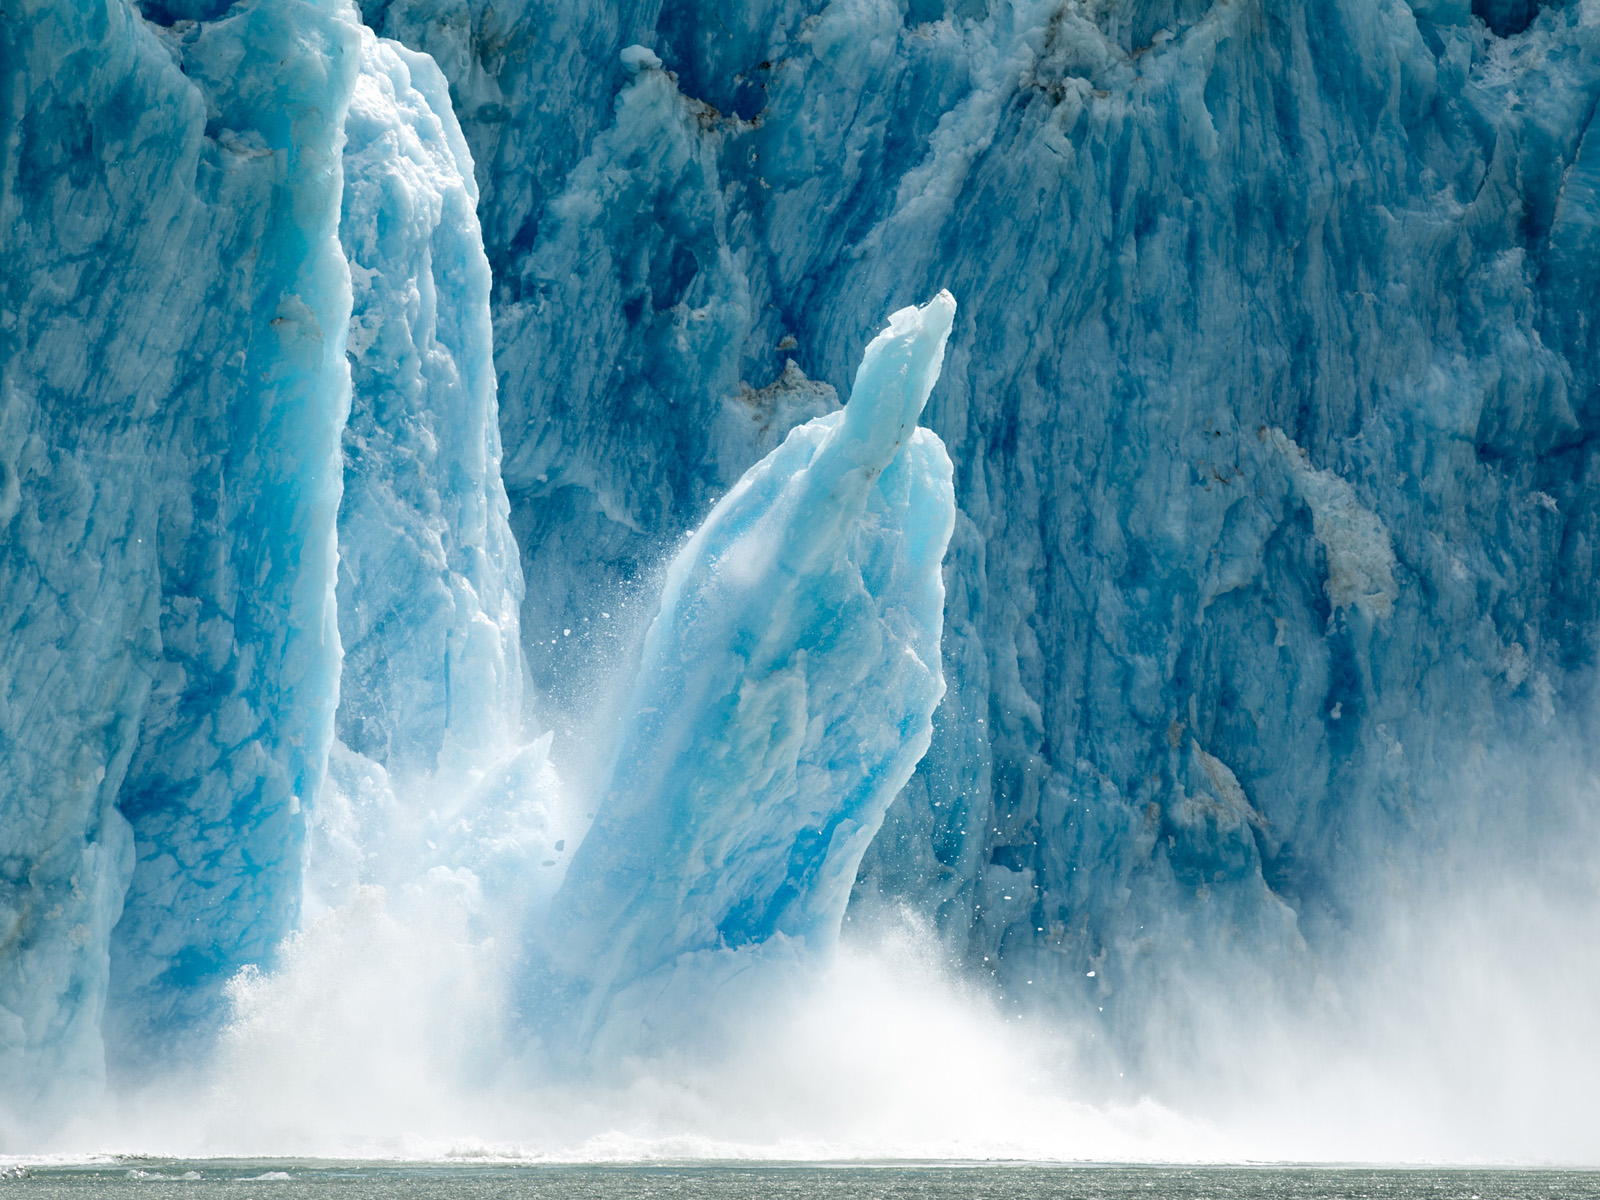
\includegraphics[height=
\paperheight,width=\paperwidth]{dawes_calving_alaska}};}
} 


\begin{frame}{The role of liquid water}
  \begin{columns}
    \column[C]{10cm}
    \begin{transbox}
      \begin{block}{at the lateral margin}
        \begin{columns}
          \column[C]{2.5cm}
          \begin{figure}
            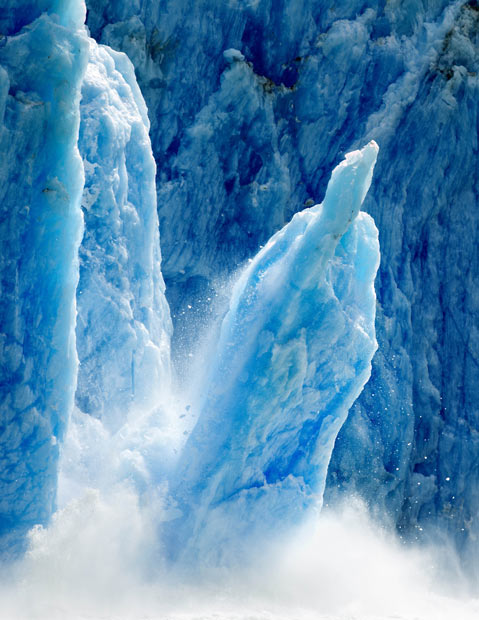
\includegraphics[width=\textwidth]{calving-close-up}
          \end{figure}
          \column[C]{7cm}
          drives calving and frontal ablation of lake and ocean terminating glaciers\\
          lecture on \alert{calving} by Doug Benn
        \end{columns}
      \end{block}
    \end{transbox}
  \end{columns}
\end{frame}

\begin{frame}{The role of liquid water}
  \begin{columns}
    \column[C]{10cm}
    \begin{transbox}
      \begin{block}{at the shelf base}
        \begin{columns}
          \column[C]{2.5cm}
          \begin{figure}
            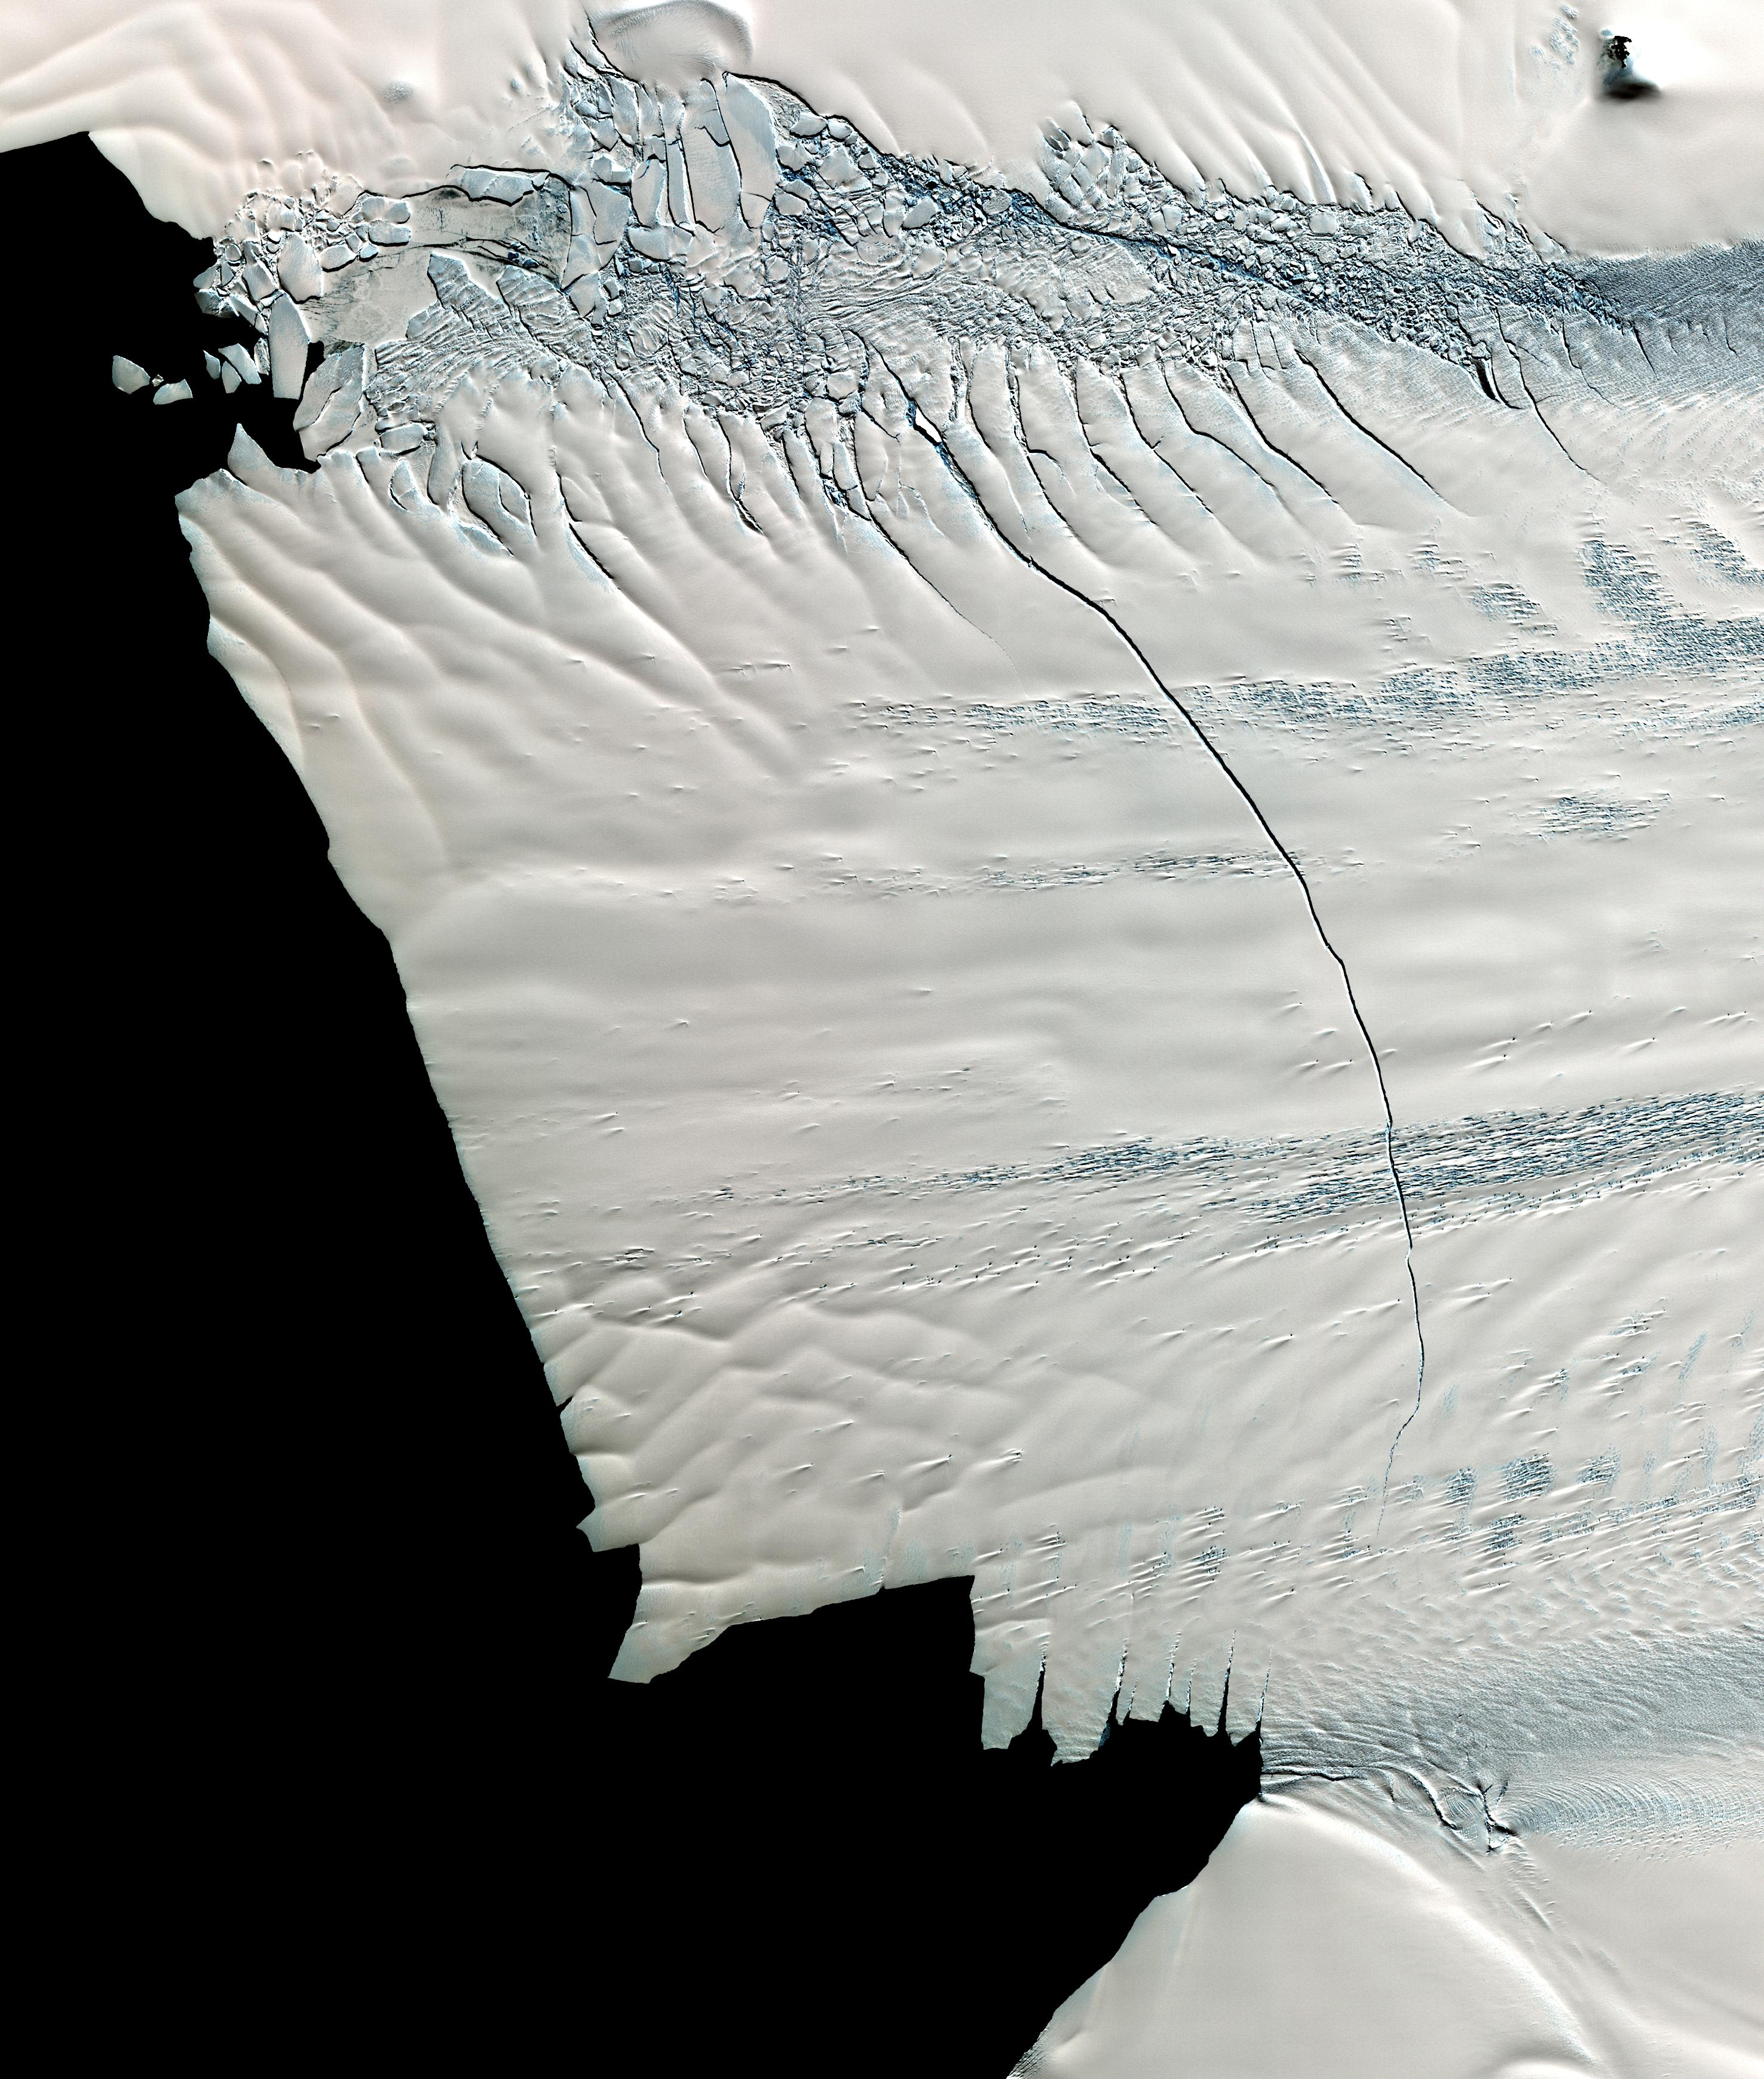
\includegraphics[width=\textwidth]{pig}
          \end{figure}
          \column[C]{7cm}
          attacks ice shelfs from below (sub-shelf basal melting) \\
          lecture on \alert{tidewater glaciers and submarine melt} by Martin Truffer
        \end{columns}
      \end{block}
    \end{transbox}
  \end{columns}
\end{frame}

\begin{frame}{The role of liquid water}
  \begin{columns}
    \column[C]{10cm}
    \begin{transbox}
      \begin{block}{at glacier base}
        \begin{columns}
          \column[C]{2.5cm}
          \begin{figure}
            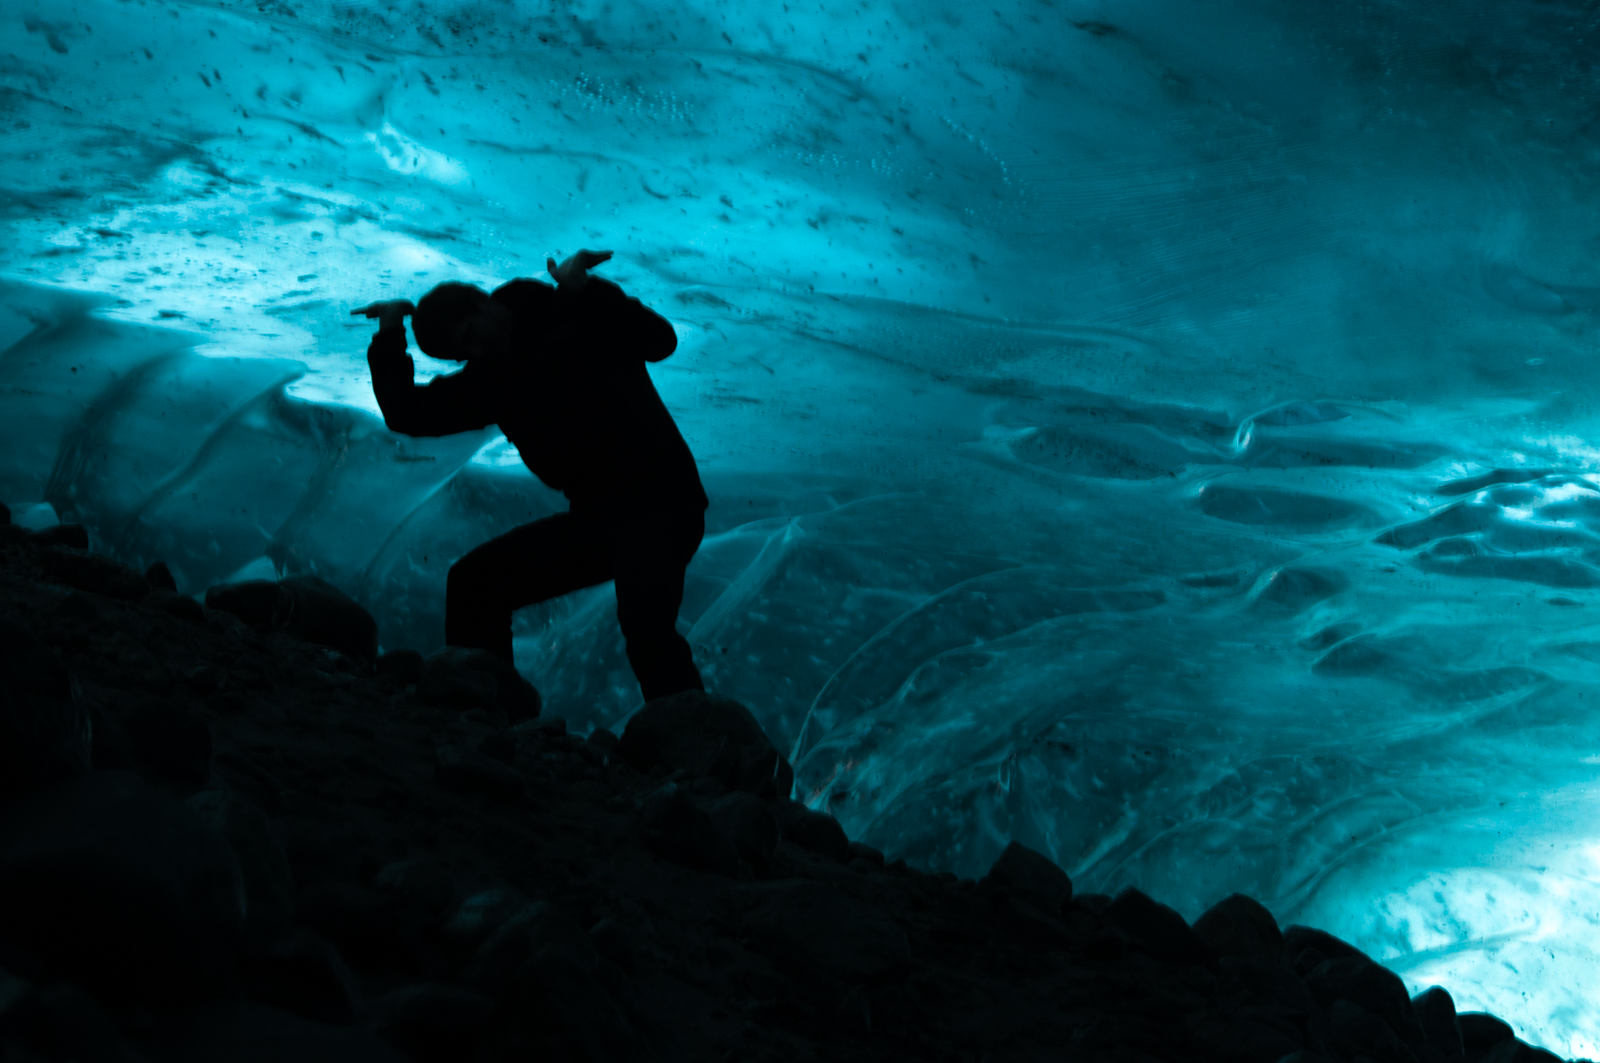
\includegraphics[width=\textwidth]{root-glacier-cave-1}
          \end{figure}
          \column[C]{7cm}
          acts as a lubricant at the base (sliding) \\
          lecture on \alert{tidewater glaciers and submarine melt} by Martin Truffer?
        \end{columns}
      \end{block}
    \end{transbox}
  \end{columns}
\end{frame}

\begin{frame}{The role of liquid water}
  \begin{columns}
    \column[C]{10cm}
    \begin{transbox}
      \begin{block}{within temperate ice}
        \begin{columns}
          \column[C]{2.5cm}
          \begin{figure}
            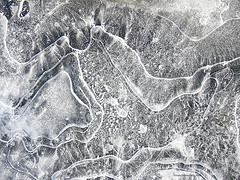
\includegraphics[width=\textwidth]{ice-matrix}
          \end{figure}
          \column[C]{7cm}
          softens the ice (decreases viscosity) \\
          lecture on \alert{thermodynamics} by Andy
        \end{columns}
      \end{block}
    \end{transbox}
  \end{columns}
\end{frame}

\setbeamertemplate{background canvas}
{
%
} 

\begin{frame}
  \frametitle{Measurements \& Observations}
    \begin{block}{1779 Gravitation theory by de~Saussure}
      H.~B. de~Saussure observes sliding
      \begin{itemize}
        \item ``\ldots the weight of the ice might be sufficient to urge it down the slope of the valley, if the sliding motion were aided by the water flowing at the bottom.''
      \end{itemize}
    \end{block}
    \begin{block}{1827-1836 Hugi Block}
      J.~Hugi observed that a boulder moved $1315\,\text{m}$ downstream between 1827 and 1836
      \begin{itemize}
        \item we would interpret this as clear evidence of glacier flow
        \item but back then, some people argued that a boulder slides on the glacier surface, the glacier itself is motionless
      \end{itemize}
    \end{block}
\end{frame}

\begin{frame}
  \frametitle{Measurements \& Observations}
  \begin{figure}
    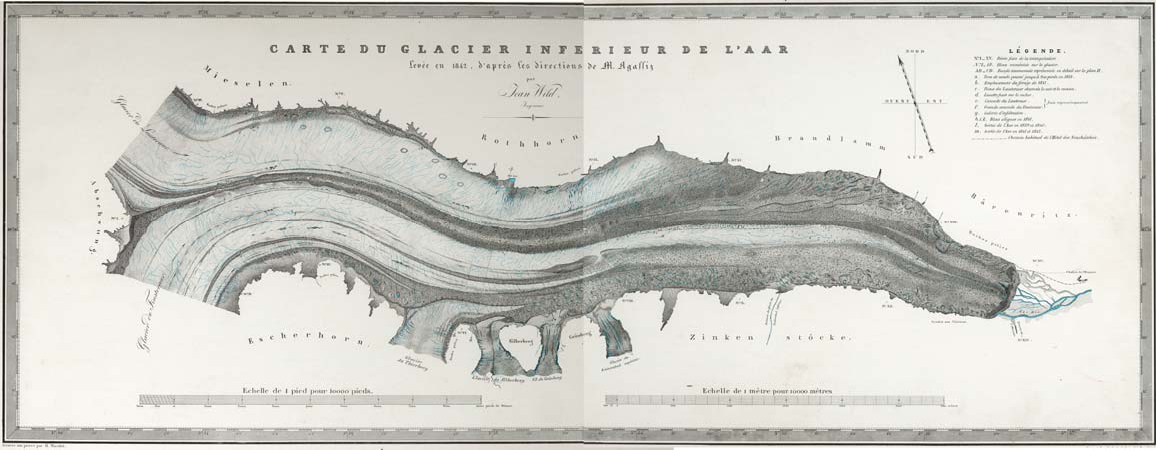
\includegraphics[width=8cm]{agassi}%
  \end{figure}
    \begin{block}{1840-1846 Dilatation theory by L. Agassiz}
      \begin{itemize}
        \item glacier ice contains innumerable fissures and capillary tubes
        \item during the day, these tubes absorb the water
        \item and during the night, the water freezes
        \item this distension exerts a force and propels the glacier in the direction of least resistance
      \end{itemize}
    \end{block}
\end{frame}


\begin{frame}
  \frametitle{Measurements \& Observations}
  \begin{columns}
    \column[C]{4.25cm}
    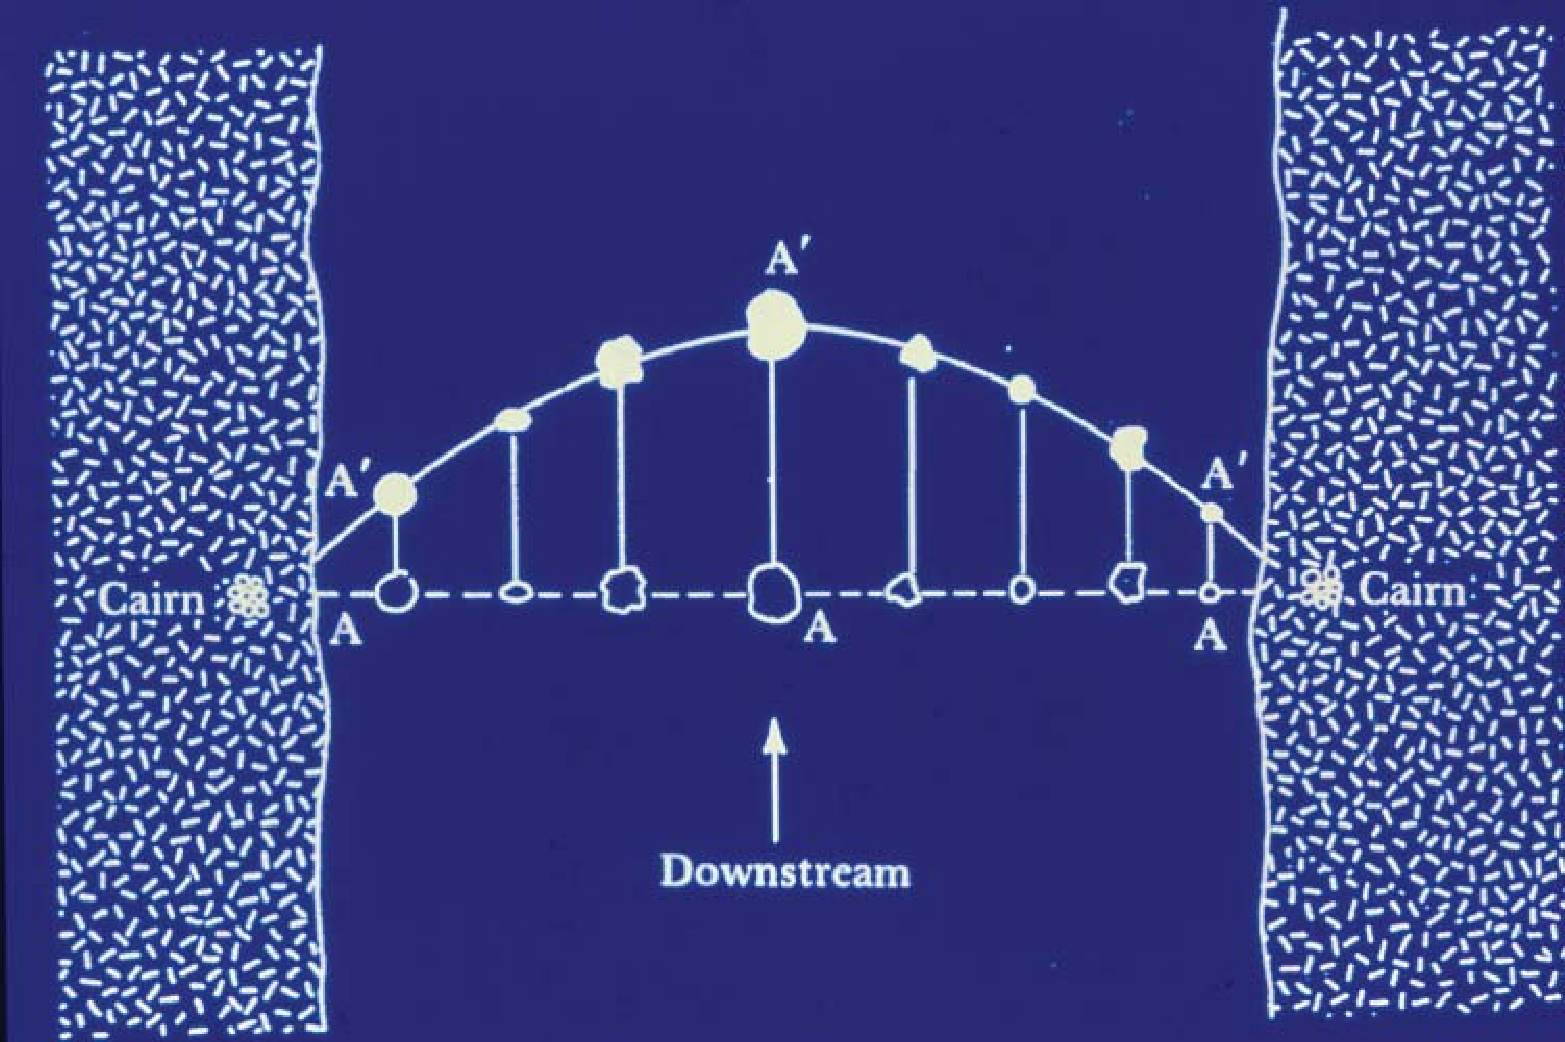
\includegraphics[width=4cm]{geschw_prof_oberfl}%
    \vskip1em
    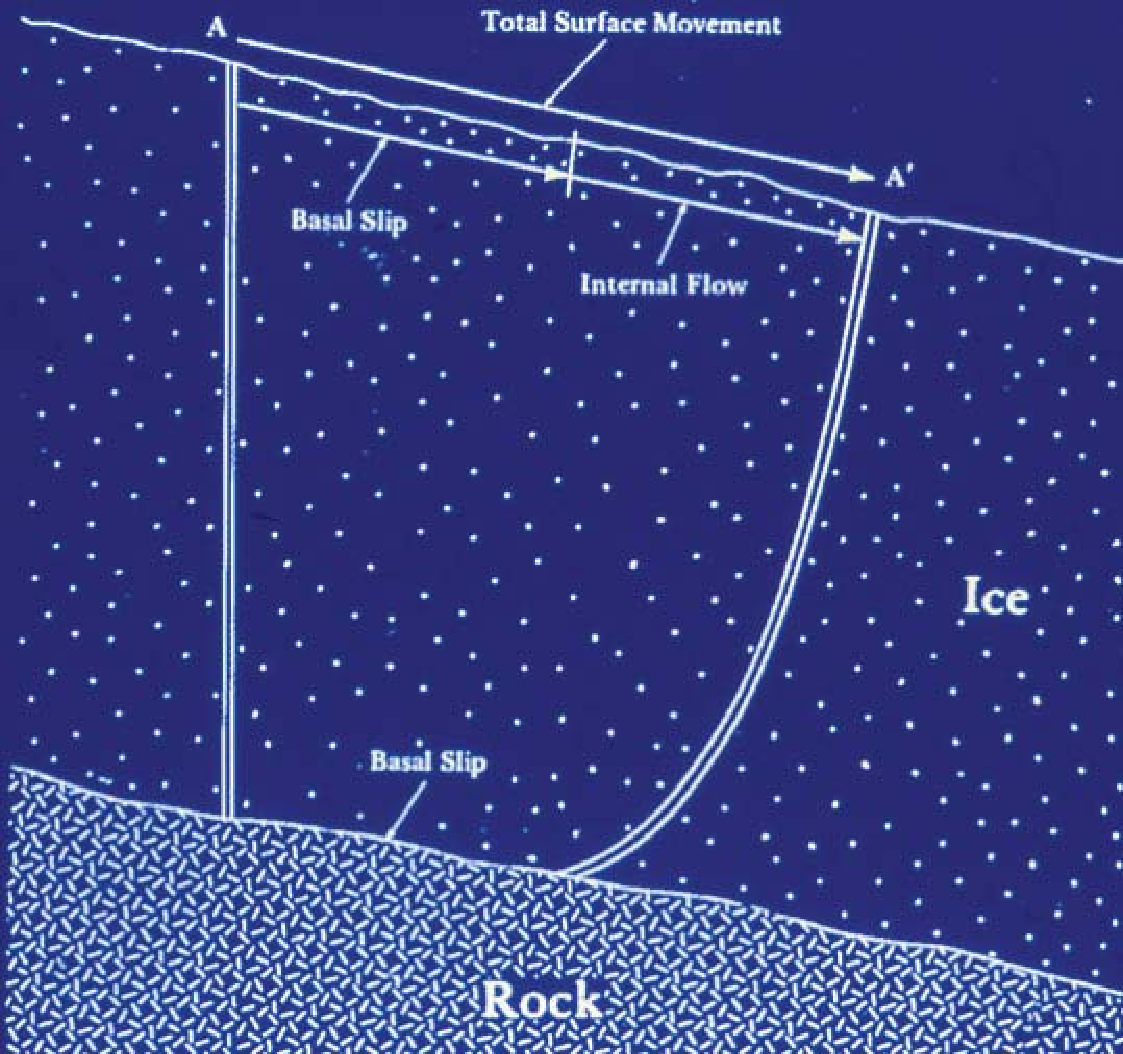
\includegraphics[width=4cm]{geschw_vert_prof}%
    \column[C]{7.75cm}
    \begin{block}{1864-1930 Viscous flow theory by J.~Forbes}
      \begin{itemize}
      \item made his own observations on Mer de Glace, France
      \item glacier flows fastest in the center
      \item opposes Agassi's theory
      \item if the dilatation theory were true
      \item then flow would be greatest at sunset
      \item and near the glacier margins
      \end{itemize}
    \end{block}
  \end{columns}
\end{frame}

\begin{frame}{Forces}
  \begin{itemize}
  \item a force is a push or pull upon an object resulting from the object's interaction with another object
  \item whenever there is an interaction between two objects, there is a force upon each of the objects. 
  \end{itemize}
  In other words
  \begin{itemize}
  \item a force is any influence that causes an object to undergo a change in speed, a change in direction, or a change in shape
  \item forces exist inside continuous bodies such as a glacier
  \item these forces can cause a glacier to deform
  \end{itemize}
\end{frame}

\begin{frame}{What is stress?}
  ``Stress'' is the force per unit area acting on a material
  \begin{displaymath}
    \sigma = \frac{F}{A}
  \end{displaymath}
  Inside a glacier, stresses are due to
  \begin{itemize}
  \item weight of the overlying ice (overburden pressure)
  \item shape of the glacier surface (pressure gradients)
  \end{itemize}
\end{frame}


\begin{frame}{Types of stress}
  As a force per unit area, stress has a direction
  \begin{columns}
    \column[c]{5cm}
    \begin{figure}
      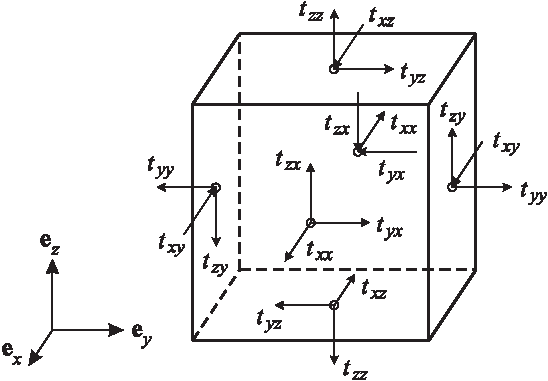
\includegraphics[width=4.75cm]{fig_3_08}
    \end{figure}
    \column[c]{6.5cm}
   \begin{block}{}
      Force can be directed normal to the area
      \begin{itemize}
      \item Result is \alert{pressure} if the force is the same on all faces of a cube.
      \item Result is \alert{normal stress} if forces are different on different faces
      \end{itemize}
    \end{block}
    \begin{block}{} 
      Force can be directed parallel to the area
      \begin{itemize}
      \item Result is \alert{shear stress}
      \end{itemize}
    \end{block}
  \end{columns}
\end{frame}

\begin{frame}{Pressure in a glacier}
  mass $m = \rho V$
     \begin{itemize}
      \item $\rho$ = ice density $\approx$ 900\,kg\,m$^{-3}$
      \item$V$ = Volume = Area $\times$ depth = $A \cdot z$
     \end{itemize}
     So pressure $p$ at depth $z$ is
     \begin{displaymath}
       p = \frac{m \cdot g}{A} = \frac{\rho \cdot A \cdot z \cdot g}{A} = \rho g z
     \end{displaymath}
     How deep do we have to drill into a glacier before the ice pressure is 1 atmosphere?
\end{frame}


\begin{frame}{Depth for 1\,atm pressure?}
    \begin{displaymath}
       z = \frac{p}{\rho\cdot g} = ?
     \end{displaymath}
     \begin{itemize}
     \item  So pressure rises by 1\,atm for every \alert{$x$}\,meters of depth in a glacier
     \item Does ice deform in response to this pressure?
     \end{itemize}
\end{frame}


\begin{frame}{Shear stress $\tau$}
  Total stress $t$ from ice column:
    \begin{displaymath}
       t = \rho V g = \rho\,g\,h
     \end{displaymath}
     \begin{itemize}
     \item How much of this weight will contribute to shear deformation?
     \item shear stress $\tau = \rho\,g\,h\,\sin{\alpha}$
     \item normal stress $\sigma = \rho\,g\,h\,\cos{\alpha}$
    \end{itemize}
\end{frame}


\begin{frame}{Shear stress in a glacier}
\begin{columns}[c]
  \begin{column}{.5\textwidth}
    \begin{block}{Valley Glacier}
      \begin{itemize}
      \item $h$ = 130\,m
      \item $\alpha$ = 5$^{\circ}$
      \end{itemize}
    \end{block}
  \end{column}
  \begin{column}{.5\textwidth}
    \begin{block}{Ice Sheet}
  \begin{itemize}
  \item $h$ = 1300\,m
  \item $\alpha$ = 0.5$^{\circ}$
  \end{itemize}
\end{block}
\end{column}
\end{columns}
\vspace{1em}
\begin{displaymath}
    \tau = \rho\,g\,h\,\sin{\alpha}
  \end{displaymath}
  \begin{beamercolorbox}[rounded=true,shadow=true]{boxed}
    Shear stress at the glacier base, $\tau_{b}$, is $\approx$ 1\,bar, which is a typical value for basal shear stress under a glacier
  \end{beamercolorbox}
\end{frame}
   

\begin{frame}{Are glacier thickness and slope related?}
  Suppose a glacier becomes thicker or steeper due to mass imbalance:
  \begin{itemize}
    \item it flows faster
    \item it quickly reduces thickness $h$ or slope $\alpha$, until $\tau_{b} \approx$ 1\,bar again
  \end{itemize}
  Can we then estimate glacier thickness ($z=h$) from its slope if we know $\tau_{b} \approx$ 1\,bar?
  \begin{displaymath}
    \tau = \rho\,g\,z\,\sin{\alpha} \quad \Rightarrow \quad h \sim \frac{\tau_{b}}{\rho\,g\,\sin{\alpha}}
  \end{displaymath}
\end{frame}


\begin{frame}{An ice sheet of infinite height?}
\begin{itemize}
  \item power-law stress-strain relationship $\Rightarrow$ ice softens
    rapidly as the shear stress exceeds 1\,bar.
  \item ice flow also increases rapidly $\Rightarrow$ glacier expands
    and thins
  \item that 1\,bar is a typical stress is a result of $A$ and $n$
\end{itemize}

\end{frame}


\begin{frame}{Parallel Sided Slab}
  \vspace{-1em}
  \begin{figure}
    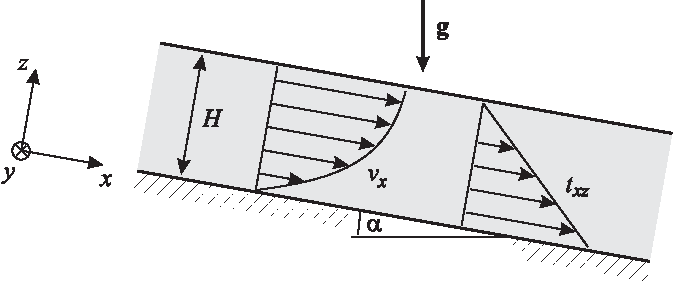
\includegraphics[width=7.5cm]{fig_3_11}
  \end{figure}
  \vspace{-1em}
  \begin{block}{Assumptions}
    \begin{itemize}
    \item uniform in x- and y-direction $\Rightarrow \partial / \partial x = \partial / \partial y = 0$
    \item steady-state $\Rightarrow \partial / \partial t = 0$
    \item stress free surface $\Rightarrow \mathbf{T}\cdot \bn \vert_{z=H} = 0$
    \item no-slip at the base $\bv \vert_{z=b} = 0$
    \end{itemize}
  \end{block}
  \vspace{.5em}
  \begin{equation*}
    \dot \varepsilon_{xz} = A\tau^{n-1} \sigma_{xz}^{(d)}
  \end{equation*}
\end{frame}

\begin{frame}{Parallel Sided Slab}
\begin{equation*}
    \begin{array}{ccl}
      \frac{\partial v_x}{\partial z}  & = &  2\,A(T,p)\,\tau^{n-1}\tau \qquad \Rightarrow \\[.5em]
      v_x (z) &  = & \int \limits_{b}^{h} 2\,A\left(\rho\,g\,\sin{\alpha}\,z\right)^{n}\,dz \\[.5em]
& = &\frac{2\,A}{n+1} \left(\rho\,g\,\sin{\alpha}\right)^{\alert{n}}\,\left(H^{\alert{n+1}} - \left(h-z\right)^{\alert{n+1}}\right)
    \end{array}
  \end{equation*}
See script p. 4--10 for a derivation
\begin{block}{Noteworthy}
\begin{itemize}
\item horizontal velocity grows with \alert{n}-th power of surface slope
\item horizontal velocity grows with \alert{n+1}-th power of ice thickness
\item this is an analytical solution, can be used for code verification (Ed's lecture)
\end{itemize}
\end{block}
\end{frame}

\begin{frame}{Flow of a Glacier in a Semi-Circular Valley}
  \vspace{-1em}
  \begin{figure}
    \centering
    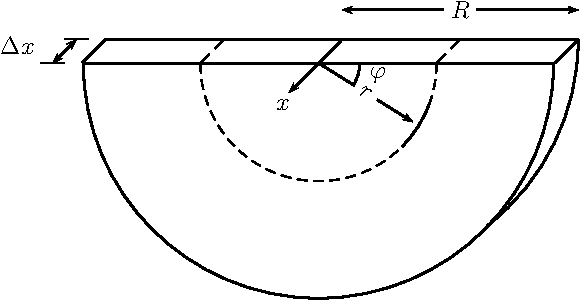
\includegraphics[width=0.4\textwidth]{fig_channel}
    \label{fig:valley-glacier-coord}
  \end{figure}
  \begin{block}{Assumptions}
    \begin{itemize}
    \item uniform in x- and $\varphi$-direction, steady-state $\Rightarrow \partial / \partial x = \partial / \partial \varphi = \partial / \partial t = 0$
    \item body force has to be balanced by tractions acting on the circumference in distance $r$ from the center
      \begin{equation*}
        \sigma_{rx} \pi r \Delta x = - \rho\,g\,\frac{\pi r^2}{2} \Delta x \sin \alpha
      \end{equation*}
\end{itemize}
  \end{block}
  \note[item]{Valley glacier: drag of the side walls}
\end{frame}

\begin{frame}{Flow of a Glacier in a Semi-Circular Valley}
 Similar to the parallel-sided slab, an analytical solution for the flow through a cylindrical channel can be obtained.
\begin{equation*}
v_x (r) = v_x (0) - \frac{2A}{n+1}\,\left( \frac{1}{2}\rho\,g\,\sin\alpha\right)^{n} r^{n+1}
\end{equation*}
\begin{block}{Noteworthy}
\begin{equation*}
v_{x, \text{channel}} = \left(\frac{1}{2}\right)^{n} v_{x, \text{slab}}
\end{equation*}
\begin{itemize}
\item here, the radius $R$ plays the role of the ice thickness $H$
\item center line velocity is \alert{eight} times slower than in an
  ice sheet of the same thickness (side wall drag)
\end{itemize}
\end{block}
\end{frame}


\begin{frame}
  \frametitle{Longitudinal Profile of a Valley Glacier}
  \begin{figure}
    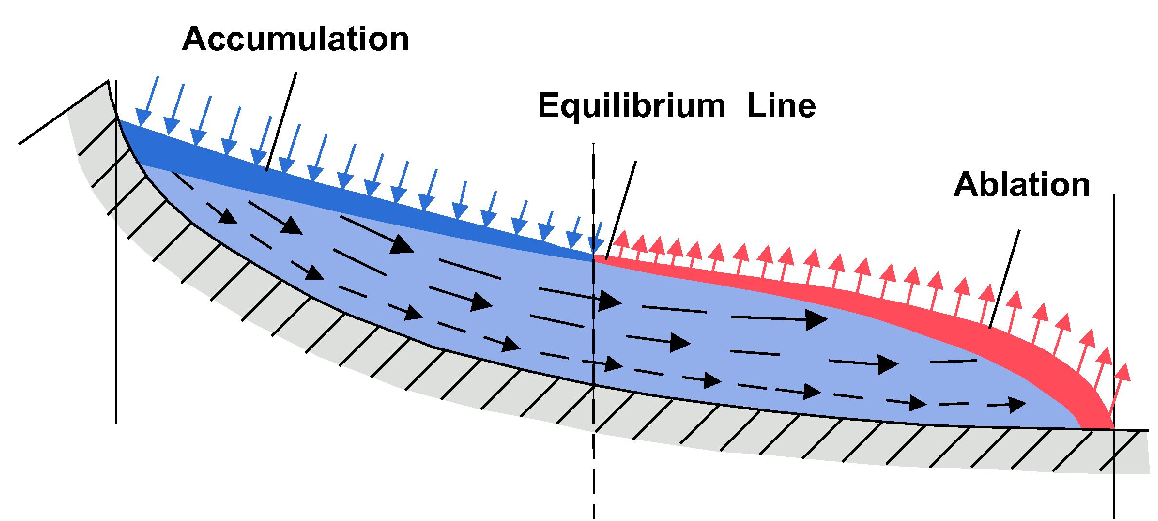
\includegraphics[width=\textwidth]{flow_acc_abl}
  \end{figure}
\end{frame}

\begin{frame}
  \frametitle{Evolution of the Glacier Surface}
  \begin{figure}
    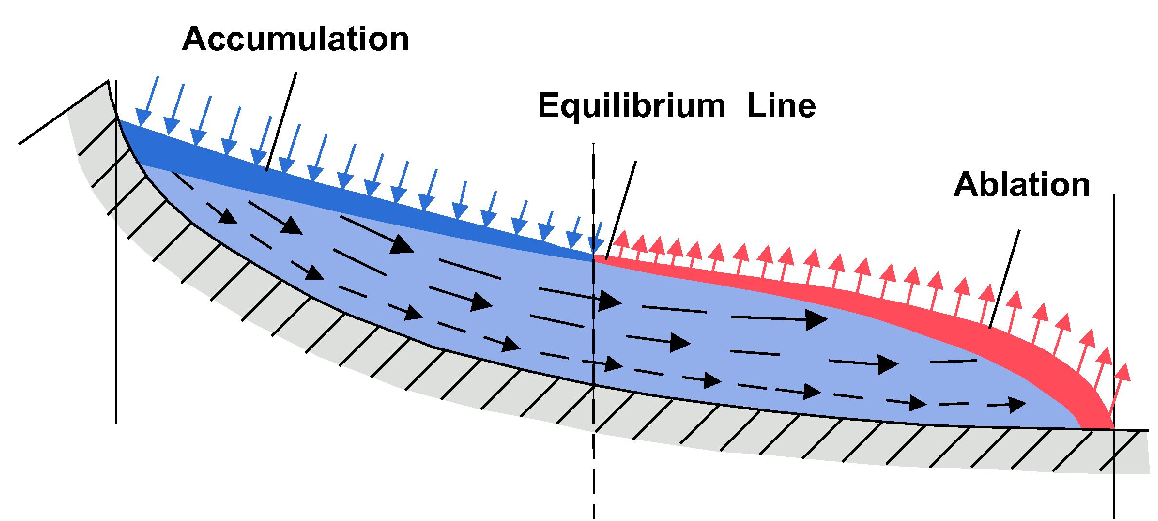
\includegraphics[width=.65\textwidth]{flow_acc_abl}
  \end{figure}
  Derivation on p. 12--14. Assuming $\partial b / \partial t = 0$ and no basal melt:
  \begin{equation*}
    \frac{\partial h}{\partial t} = - \underbrace{\nabla \cdot \mathbf{Q}}_{\text{dynamic changes}} + \underbrace{a_{\text{s}}}_{\text{climatic changes}}
  \end{equation*}
\end{frame}


\begin{frame}{Why is it so hard to predict the future of an ice
    sheet?}
  \begin{block}{It's easy because}
   \begin{itemize}
    \item composed of a single, largely homogenous material
    \item viscous flow is governed by the Navier-Stokes equations (19th century physics)
    \item move very slowly (turbulence, Coriolis force, and other inertial effects can be ignored)
   \end{itemize}
  \begin{beamercolorbox}[rounded=true,shadow=true]{boxed}
``I am an old man now, and when I die and go to heaven there are two matters on which I hope for enlightenment. One is quantum electrodynamics, and the other is the turbulent motion of fluids. And about the former I am rather optimistic.'' (O.~Reynolds)
  \end{beamercolorbox}

  \end{block}
\end{frame}

\begin{frame}{Why is it so hard to predict the future of an ice
    sheet?}
  \begin{block}{It's so hard because}
   \begin{itemize}
    \item the stress resisting ice flow at the base can vary by orders of magnitude
    \item ocean interactions could trigger instabilities
    \item difficult to observe boundary conditions $\Leftarrow$ \alert{inverse methods} lecture by Martin Truffer
  \end{itemize}
  \end{block}
  \begin{figure}
    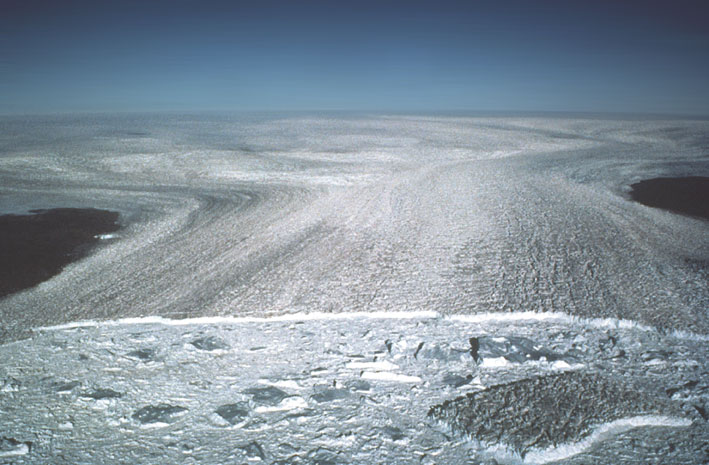
\includegraphics[width=4cm]{jakobshavn_calving}
  \end{figure}
\end{frame}

\begin{frame}{Now and then}
  \begin{columns}
    \column[c]{6cm}
    \begin{figure}
      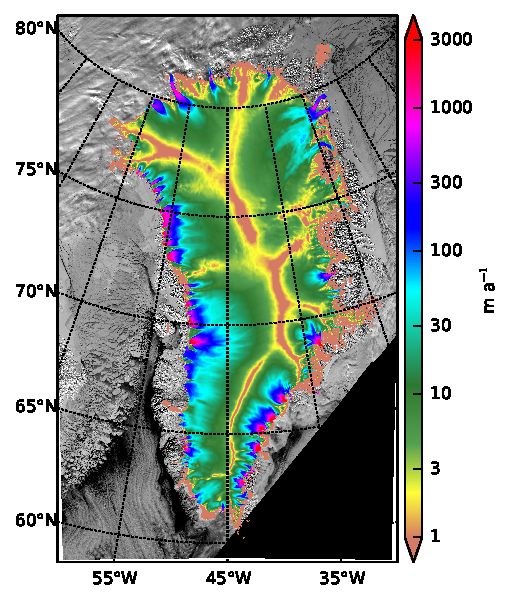
\includegraphics[height=7.5cm]{today}
    \end{figure}
    \column[c]{6cm}
    \begin{itemize}
      \item model physics is better
      \item grid resolution is finer
      \item spatially-rich time-series of a multitude of observables is available for forcing and validation
    \end{itemize}
  \end{columns}
\end{frame}

\begin{frame}{Now and then}
  \begin{columns}
    \column[c]{8cm}
    \begin{figure}
      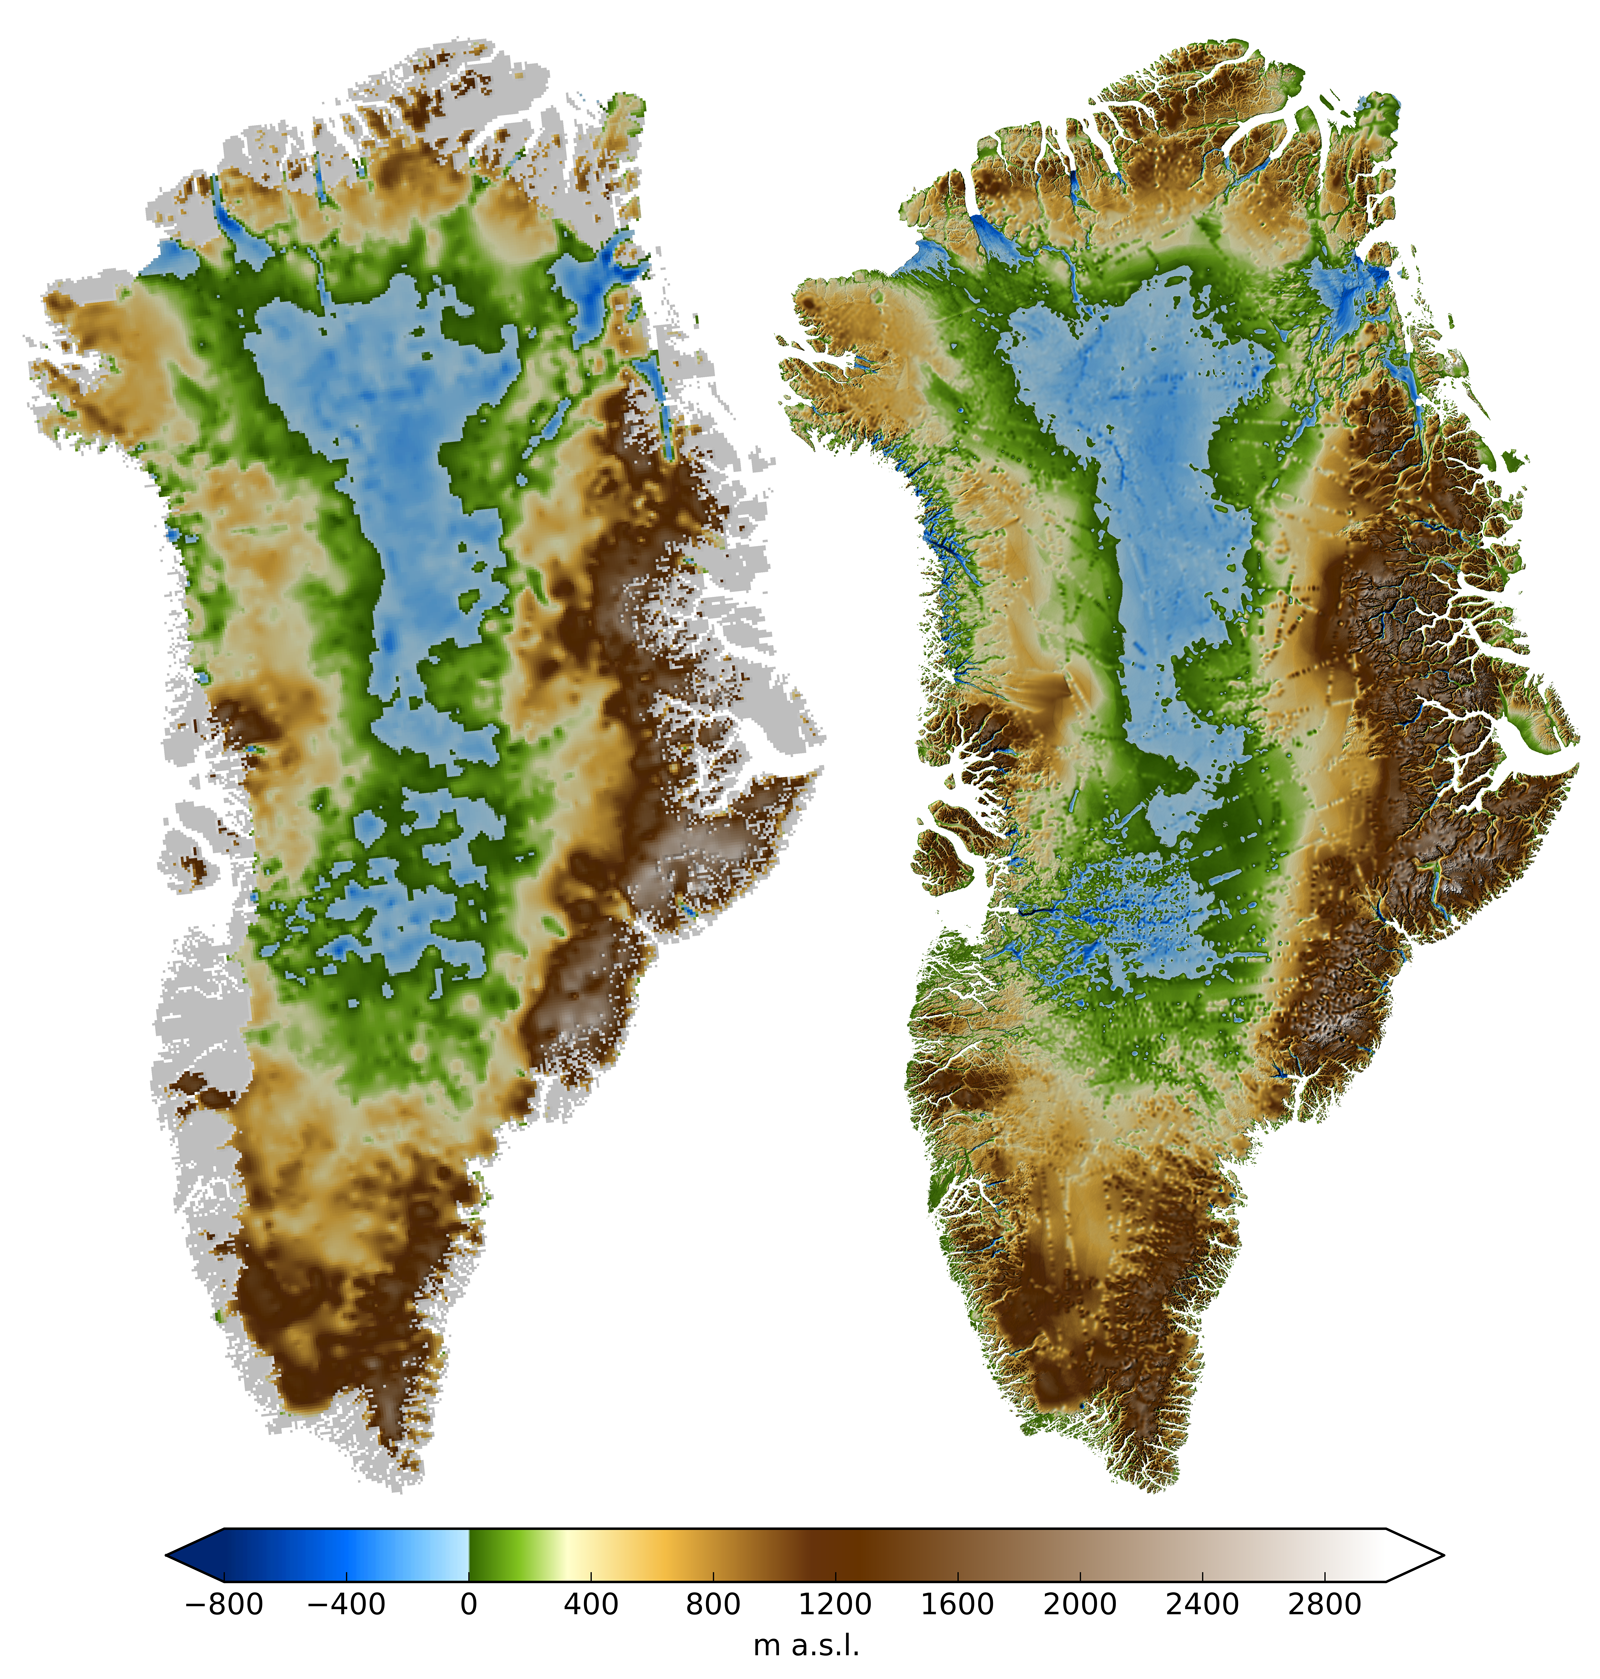
\includegraphics[height=8cm]{greenland_bed}
    \end{figure}
    \column[c]{4cm}
    \begin{itemize}
    \item from 5\,km to 150\,m horizontal grid resolution
    \end{itemize}
  \end{columns}
\end{frame}

\begin{frame}{Now and then}
  \begin{figure}
    Bamber (2001) \hspace{4em} Morlighem (2014)
    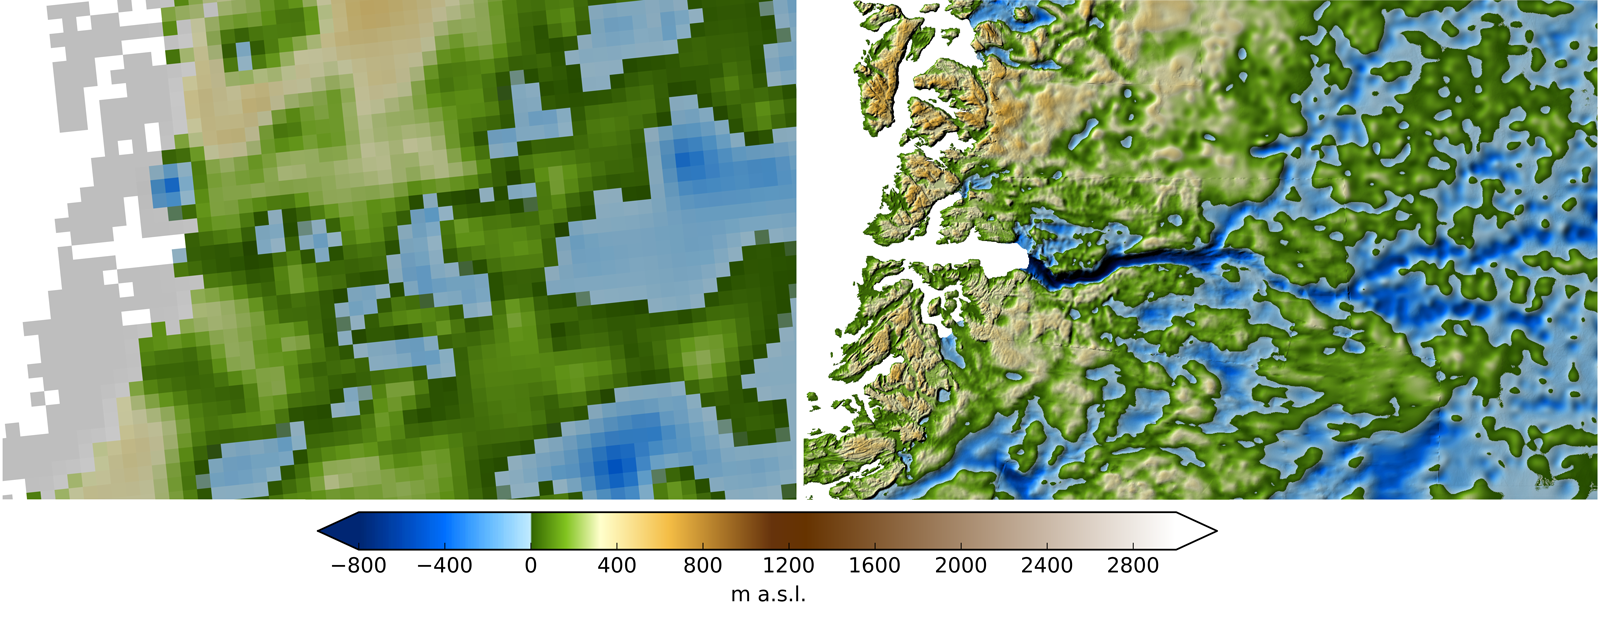
\includegraphics[width=12cm]{jako_bed}
 \end{figure}
\end{frame}


\begin{frame}{Now and then}
      \begin{figure}
        \includegraphics[height=6.5cm]{greenland-sar-ar4-today}
     \end{figure}
\end{frame}

\end{document}
